\documentclass[12pt,a4paper]{article}
\usepackage[T1]{fontenc}\usepackage[utf8]{inputenc}\usepackage{times}
\usepackage[a4paper,top=2.5cm,bottom=2.5cm,left=2.5cm,right=2.5cm]{geometry}
\usepackage{graphicx}
\graphicspath{{figures/}}
\usepackage{booktabs}\usepackage{array}\usepackage{enumitem}\usepackage{tabularx}
\usepackage{caption}\usepackage{fancyhdr}\usepackage{parskip}\usepackage{float}
\usepackage{setspace}\onehalfspacing
\usepackage{amsmath}
\usepackage{xurl}\usepackage[hidelinks]{hyperref}
\captionsetup{font=small,labelfont=bf,labelsep=colon,
              justification=justified,singlelinecheck=false}
\setlist[itemize]{leftmargin=1.3em,itemsep=0pt,parsep=0pt,topsep=2pt}
\setlist[enumerate]{leftmargin=1.6em,itemsep=0pt,parsep=0pt,topsep=2pt}
\setlength{\parskip}{4pt plus 1pt}
\renewcommand{\topfraction}{0.85}\renewcommand{\bottomfraction}{0.7}\renewcommand{\textfraction}{0.1}\renewcommand{\floatpagefraction}{0.75}
\pagestyle{fancy}\fancyhf{}
\fancyhead[L]{\footnotesize KOUAME Koffi Fid\`ele}
\fancyhead[C]{\footnotesize MOVIE ANALYTICS}
\fancyhead[R]{\footnotesize Data Analysis Internship}
\fancyfoot[C]{\thepage}\renewcommand{\headrulewidth}{0.4pt}
\setlength{\headheight}{15pt}
\newcommand{\fig}[2]{\begin{figure}[H]\centering\includegraphics[width=0.84\linewidth]{#1}\caption{#2}\end{figure}}

\begin{document}

\begin{titlepage}\centering
\singlespacing
\vspace*{3cm}
{\large\scshape Data Analysis Internship}\\[0.4cm]
{\normalsize Task 10}\\[2.0cm]
\rule{\linewidth}{0.5pt}\\[0.8cm]
{\LARGE\bfseries Movie Analytics Dashboard}\\[0.6cm]
{\large What Drives the Success of a Film?\\ A Power BI Story on 3{,}754 TMDB Movies}\\[0.8cm]
\rule{\linewidth}{0.5pt}\\[1.2cm]
{\normalsize Data Model $\bullet$ KPIs $\bullet$ Genres and Ratings $\bullet$ Box Office
$\bullet$ Runtime $\bullet$ Trends $\bullet$ Interactive Dashboard}\\[3.2cm]
{\large\itshape Prepared by}\\[0.5cm]
{\Large\bfseries KOUAME Koffi Fid\`ele}\\[0.6cm]
{\large 3 October 2026}
\vfill\end{titlepage}

\singlespacing
\tableofcontents\newpage
\onehalfspacing

% =====================================================================
\section{Executive summary}

The brief asks for an interactive Power BI dashboard that analyses movie data and
tells a clear story about the trends and factors related to movie success. This
report presents the analysis behind each visual, the data model and the design of
the dashboard; the notebook \texttt{Movie-Analytics.ipynb} reproduces every number
and figure, and the folder \texttt{powerbi/} contains the dashboard
(\texttt{Movie\_Analytics\_Dashboard.pbix}, with the data loaded), its template
(\texttt{Movie\_Analytics\_Dashboard.pbit}), the theme, the DAX measures and the build
guide. In the dashboard, the supplied file is loaded as it was received and transformed
step by step in Power Query, so the whole path from \texttt{tmdb\_5000\_credits.csv} to
every visual can be inspected in Power BI.

\textbf{Data.} The supplied file, \texttt{tmdb\_5000\_credits.csv}, is the primary source:
it fixes the list of films and provides their titles, cast and crew (4{,}803 films). It
contains none of the attributes the brief asks to analyse (year, genres, budget,
revenue, rating, votes, runtime). These come from a second, public source, TMDb Movies,
joined on the TMDb identifier: \textbf{3{,}754 films (78.2\%)} of the supplied file,
released between 1960 and 2015, are analysed; the unmatched films are mostly 2016
releases.

\textbf{Key figures.} The 3{,}754 films earned \textbf{\$369.5 billion} for
\textbf{\$130.0 billion} of declared budgets. Among the 2{,}805 films with both values
known, the median film returns \textbf{2.27 times} its budget and \textbf{76.6\%}
recover it. The average rating is \textbf{6.13 out of 10} and the average runtime
\textbf{109 minutes}.

\textbf{Main findings.}
\begin{itemize}
\item \textbf{Money buys revenue, not acclaim.} Budget and revenue are strongly
related (Spearman $\rho = 0.65$); budget and rating are not ($\rho = -0.08$).
\item \textbf{Genre shapes the rating}: Documentary (6.73), War (6.63) and History
(6.55) are the best rated, Horror (5.66) the lowest.
\item \textbf{Longer films are better rated and earn more}: from 5.69 under 90 minutes to
6.93 above 150 minutes, and median revenue triples.
\item \textbf{The box office is ruled by recent franchise blockbusters} (Avatar,
The Avengers, Jurassic World); the best films, once the vote count is considered, are
classics with thousands of votes (The Shawshank Redemption, The Dark Knight, The
Godfather).
\item \textbf{The typical film is not richer than thirty years ago} in inflation-adjusted
dollars, and average ratings drift down slightly over time.
\end{itemize}

% =====================================================================
\section{Data and method}

\subsection{Two sources: the supplied file and a required enrichment}

\textbf{Source 1, supplied: \texttt{tmdb\_5000\_credits.csv}.} This is the file received
for the task. It is one of the two files of the Kaggle \emph{TMDB 5000 Movie Dataset}
(reference~1), hence its name. It defines the population of the study (4{,}803 films,
identified by \texttt{movie\_id}) and is the only source of the titles, actors and
directors used in the dashboard.

\textbf{Source 2, enrichment: \texttt{tmdb-movies.csv}.} The brief asks to analyse
release years, genres, ratings, budgets, revenues and runtimes. Table~\ref{tab:coverage}
shows that the supplied file contains none of them: without a second source, none of the
requirements R1 to R8 could be answered, only rankings of actors and directors by number
of films. The public TMDb Movies dataset
(reference~2) comes from the same database (TMDb) and uses the same identifier, so the
two files can be joined without any fuzzy matching.

\begin{table}[H]\centering\small
\caption{Which source answers each requirement of the brief.}\label{tab:coverage}
\begin{tabularx}{\linewidth}{@{}Xcc@{}}
\toprule
Attribute needed by the brief & Source 1 (supplied) & Source 2 (enrichment)\\\midrule
Film identifier and title & yes & yes\\
Actors, directors (People page) & yes & no\\
Release year and date (R1, R7) & no & yes\\
Genres (R2, R3) & no & yes\\
Budget and revenue, nominal and 2010 \$ (R4, R5, R7) & no & yes\\
Rating and vote count (R3, R6, R7) & no & yes\\
Runtime (R8) & no & yes\\
\bottomrule
\end{tabularx}
\end{table}

\begin{table}[H]\centering\small
\caption{The two data sources and the join.}
\begin{tabularx}{\linewidth}{@{}lXr@{}}
\toprule
File & Content & Films\\\midrule
Source 1: \texttt{tmdb\_5000\_credits.csv} (supplied) & cast and crew in JSON: actors, billing order, directors & 4{,}803\\
Source 2: \texttt{tmdb-movies.csv} (public enrichment) & year, genres, budget, revenue (nominal and 2010 \$), rating, votes, runtime & 10{,}866\\
Inner join on \texttt{movie\_id = id} & films of Source 1 found in Source 2 & \textbf{3{,}754}\\
\bottomrule
\end{tabularx}
\end{table}

The join is reliable: 98.3\% of the matched films have identical titles, the others
carrying their original-language title in the enrichment. The dashboard uses the
titles of the supplied file. The companion file of the supplied one,
\texttt{tmdb\_5000\_movies.csv} (same Kaggle dataset), would provide the same attributes
for all 4{,}803 films including 2016; it was not supplied, and the Power Query
pipeline is written so that it can replace Source 2 by changing a single step.

\subsection{Cleaning decisions}

\begin{itemize}
\item \textbf{Zero means unknown.} 564 budgets, 828 revenues and 2 runtimes equal to 0
become missing values. Financial indicators use the 2{,}805 films with both budget
and revenue known.
\item \textbf{Inflation.} Comparisons across years use the inflation-adjusted
revenues (2010 dollars).
\item \textbf{Weighted rating.} 22.6\% of the films have fewer than 50 votes. Films are
ranked with the Bayesian average used by IMDb,
\[ WR = \frac{v}{v+m}\,R + \frac{m}{v+m}\,C, \]
where $R$ is the film's rating, $v$ its votes, $C = 6.13$ the mean rating and
$m = 1{,}354$ the 90th percentile of the vote counts.
\item \textbf{Multi-valued fields.} Genres (2.65 per film), the five first-billed
actors and the directors are unpacked into bridge tables.
\end{itemize}

\subsection{From the supplied file to the Power BI model}

The whole preparation runs inside Power BI, in Power Query (Figure~\ref{fig:pipeline}).
The two CSV files are read from a folder set by the parameter \texttt{DataFolder}; every
step is visible in \emph{Transform data}, in the Applied Steps of each query, so a
reader can check how each number of the dashboard is obtained from the supplied file.
The notebook performs the same steps in Python and gives the same results.

\begin{figure}[H]\centering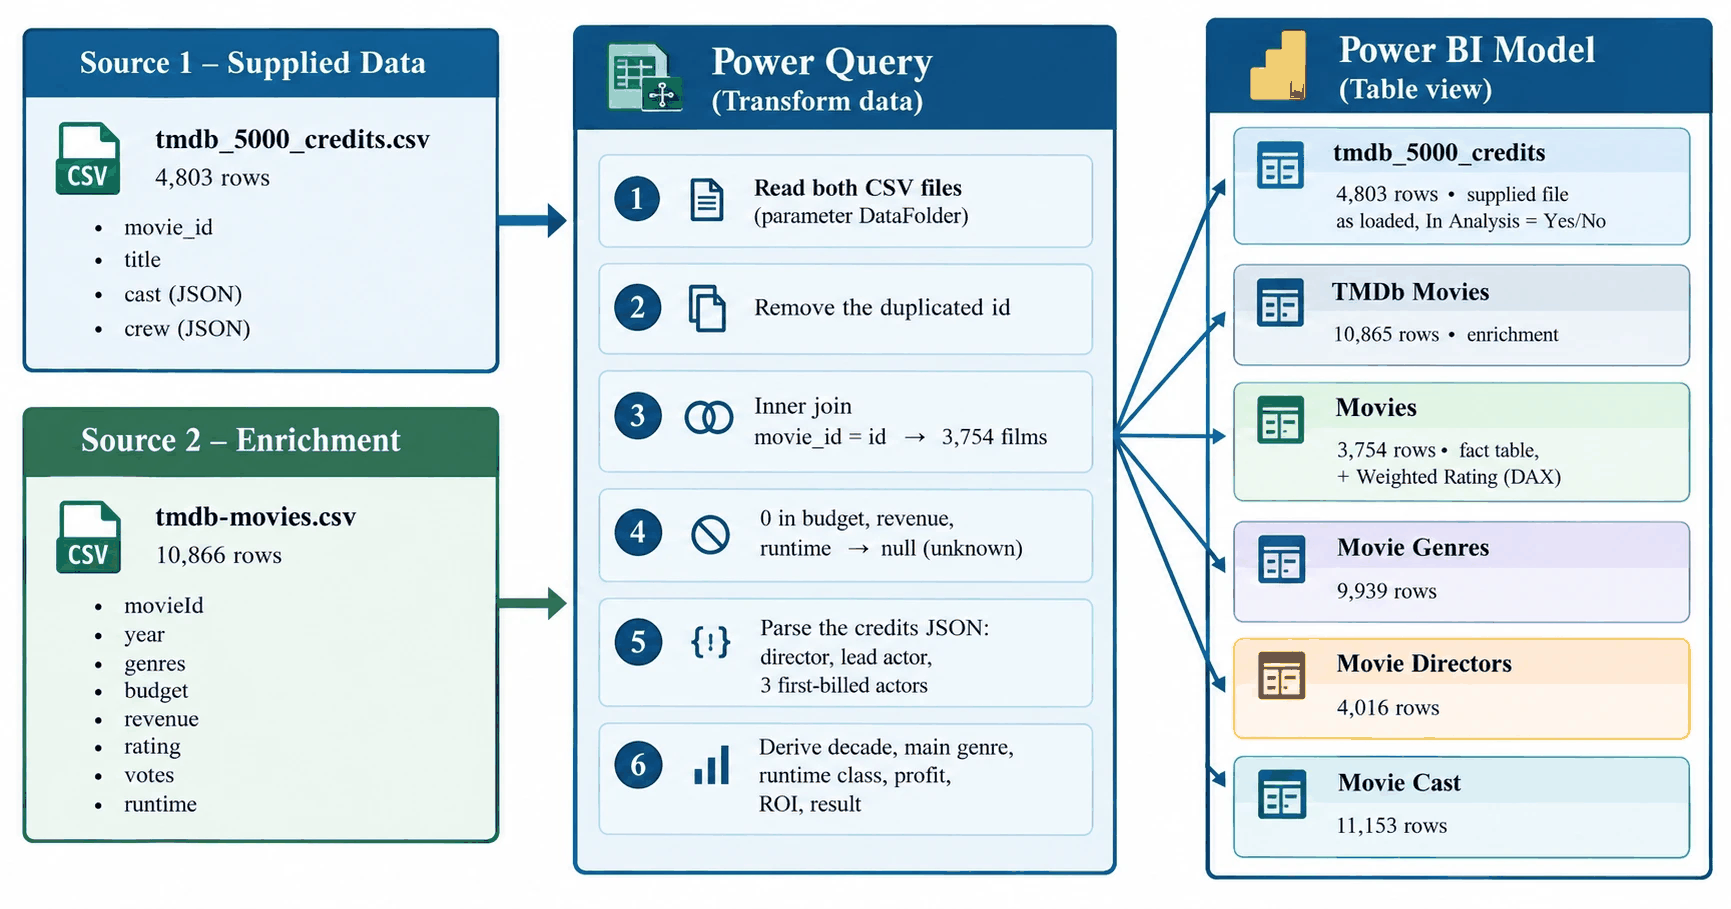
\includegraphics[width=\linewidth]{fig10_data_pipeline.png}
\caption{Data pipeline of the dashboard: the supplied file (Source 1) is enriched by
TMDb Movies (Source 2) in Power Query, which produces the six tables of the model.}
\label{fig:pipeline}\end{figure}

\begin{table}[H]\centering\small
\caption{Tables of the Power BI model, as listed in the Table view.}
\begin{tabularx}{\linewidth}{@{}lrX@{}}
\toprule
Table & Rows & Content\\\midrule
\texttt{tmdb\_5000\_credits} & 4{,}803 & the supplied file as received: \texttt{movie\_id}, title, number of cast and crew members, and \emph{In Analysis} (Yes for the 3{,}754 films found in Source 2)\\
\texttt{TMDb Movies} & 10{,}865 & the enrichment, after removal of one duplicated identifier\\
\texttt{Movies} & 3{,}754 & fact table, one row per analysed film: year, date, decade, genres, director, lead actor, financials, profit, ROI, result, rating, votes, runtime class, weighted rating\\
\texttt{Movie Genres} & 9{,}939 & one row per film and genre\\
\texttt{Movie Directors} & 4{,}016 & director(s) of each film, from the crew of Source 1\\
\texttt{Movie Cast} & 11{,}153 & three first-billed actors of each film, from the cast of Source 1\\
\bottomrule
\end{tabularx}
\end{table}

\textbf{Why the analysis tables are separate from the supplied file.} The cast and crew
columns of \texttt{tmdb\_5000\_credits} hold one JSON text per film, with up to several
hundred people inside; Power BI cannot count, filter or rank what is inside such a text.
Power Query therefore unpacks them into \texttt{Movie Directors} and \texttt{Movie Cast},
one row per person and film, and keeps \texttt{tmdb\_5000\_credits} in the model as the
reference of what was received. The page \emph{Data Pipeline} of the dashboard
(Figure~\ref{fig:p7}) shows this table, its 4{,}803 films and the share kept in the analysis.

\textbf{Relationships.} \texttt{Movies[Movie ID]} is linked one-to-many to the three bridge
tables, with a cross-filter direction set to \emph{Both}, so that a genre, actor or
director selection filters the films. \texttt{tmdb\_5000\_credits} and \texttt{TMDb Movies}
are linked to \texttt{Movies} on the identifier, which documents the lineage in the
Model view.

% =====================================================================
\section{Key performance indicators}

\begin{table}[H]\centering\small
\caption{The eight KPI cards of the Home page (no filter applied).}
\begin{tabularx}{\linewidth}{@{}lrX@{}}
\toprule
KPI & Value & Base\\\midrule
Movies & 3{,}754 & all matched films\\
Total revenue & \$369.5 bn & films with known revenue\\
Total budget & \$130.0 bn & films with known budget\\
Median ROI (revenue / budget) & 2.27x & films with known budget and revenue (2{,}805)\\
Profitable films & 76.6\% & films with known budget and revenue\\
Average rating & 6.13 / 10 & all films\\
Average runtime & 109 min & films with known runtime\\
Total votes & 1{,}912{,}799 & all films\\
\bottomrule
\end{tabularx}
\end{table}

Films with known financials are mostly the larger, better-documented productions;
the profitability figures describe the commercial cinema of the dataset rather than
every film produced. These eight cards open the Home page of the dashboard
(Figure~\ref{fig:p1}).

% =====================================================================
\section{Results}

\subsection{Movies released over the years (R1)}
\fig{fig01_films_per_year.png}{Films per release year. Production rises from a few
films a year in the 1960s to 150--200 after 2000, with a peak of 197 in 2009.}

72\% of the films were released after 2000. The rise reflects both the growth of
production and the better documentation of recent films by TMDb users; decades must
therefore be compared with averages or medians, never totals. In the dashboard, this
chart opens the page \emph{Releases \& Genres} (Figure~\ref{fig:p2}).

\subsection{Movies by genre (R2)}
\fig{fig02_films_per_genre.png}{Films per genre. Drama, Comedy, Thriller and Action
dominate; a film has 2.65 genres on average, so the bars add up to more than 3{,}754.}

\subsection{Average ratings across genres (R3)}
\fig{fig03_rating_by_genre.png}{Average rating by genre (genres with at least 50 films),
with 95\% confidence intervals. The dashed line is the average of all films (6.13).}

Documentary, War, History, Music, Western and Drama are rated above average; Horror is
clearly the lowest (5.66), followed by Comedy, Science Fiction and Action (about 6.0).
The genre effect is significant (Kruskal--Wallis $H = 626$, $p < 10^{-100}$) but
spans only about one point on the ten-point scale. The dashboard shows the same ranking
on the page \emph{Releases \& Genres} (Figure~\ref{fig:p2}, lower left).

\subsection{Budget and revenue (R4)}
\fig{fig04_budget_vs_revenue.png}{Budget against worldwide revenue, logarithmic scales.
Films above the dashed line recover their budget (green), films below do not (red).}

\begin{table}[H]\centering\small
\caption{Return on investment by budget class (films with known financials).}
\begin{tabular}{@{}lrrrr@{}}
\toprule
Budget class & Films & Median revenue (\$M) & Median ROI & Profitable\\\midrule
$<$ \$10M & 568 & 13.9 & 3.39 & 76\%\\
\$10--30M & 926 & 41.8 & 2.17 & 74\%\\
\$30--70M & 793 & 95.0 & 1.98 & 75\%\\
\$70--150M & 424 & 237.5 & 2.29 & 82\%\\
$>$ \$150M & 94 & 554.9 & 2.85 & 95\%\\
\bottomrule
\end{tabular}
\end{table}

Bigger budgets bring bigger revenues ($\rho = 0.65$) and fewer failures, but not a
better return: the median ROI is highest for small films (3.4x below \$10M). The page
\emph{Box Office} of the dashboard (Figure~\ref{fig:p3}) shows the same scatter for each
film, with the median ROI by main genre: Horror (3.35x) and Science Fiction (3.10x) lead.

\subsection{Highest-grossing movies (R5)}
\fig{fig05_top_grossing.png}{Top 10 films by worldwide revenue (nominal dollars), with
their budget (grey bar) and return on investment.}

Avatar (\$2.78 bn), Titanic (\$1.85 bn) and The Avengers (\$1.52 bn) lead. All are
franchise or animation blockbusters released after 2009, except Titanic, and each
returns 5 to 16 times its budget (Figure~\ref{fig:p3}, top right). In 2010 dollars, older hits enter the top 10:
Star Wars (1977), The Exorcist (1973), Jaws (1975) and E.T. (1982).

\subsection{Highest-rated movies considering the vote count (R6)}
\fig{fig06_top_rated.png}{Top 10 films by weighted rating. The raw rating and the
number of votes are given for each film.}

On the raw rating, a film rated 8.4 by 11 users ties with The Shawshank Redemption
(8.4 from 5{,}754 users). The weighted rating removes this artefact: the top 10 are
all films with thousands of votes. The same ranking is the table of the page
\emph{Ratings \& Runtime} (Figure~\ref{fig:p4}), sorted by weighted rating.

\subsection{Revenue and ratings over the years (R7)}
\fig{fig07_trends.png}{(a) Median revenue per film, inflation-adjusted and nominal;
(b) average rating per film. Years with at least 20 films.}

In 2010 dollars, the median film falls from about \$136M in the 1970s to \$81--84M in
the 1980s--1990s and \$67--68M after 2000; nominal growth is mostly inflation. The
average rating drifts from about 6.6 for films of the 1960s--1970s to 6.0--6.1 after
2000 ($\rho = -0.09$), partly because the old films kept in the database are the
classics that people still watch and rate.

\subsection{Runtime, ratings and revenue (R8)}
\fig{fig08_runtime.png}{(a) Runtime distribution (median 105 minutes); (b) average
rating and (c) median revenue by runtime class.}

Ratings rise steadily with length, from 5.69 below 90 minutes to 6.93 above 150 minutes
($\rho = 0.38$), and the median revenue triples from about \$45M to \$135M
($\rho = 0.25$). This is an association: long films are more often prestige dramas,
epics and blockbusters; length alone does not make a film better. The two runtime
charts of Figure~\ref{fig:p4} exclude the two films of unknown runtime.

\subsection{Complement: directors and actors (from the supplied credits)}
\fig{fig09_top_directors.png}{Top 10 directors by total worldwide revenue (at least five
films with known financials).}

Steven Spielberg (\$9.0 bn, 26 films), Peter Jackson and James Cameron lead; Christopher
Nolan combines box office with the best average rating (7.64). The most frequent
actors in the first five billings are Robert De Niro (51 films), Samuel L. Jackson (41)
and Bruce Willis (39). The dashboard counts the three first-billed actors only, the
leading roles: Robert De Niro (44), Bruce Willis (35), Matt Damon and Nicolas Cage (34).
Its ranking of the best-rated directors uses the weighted rating and directors with at
least three films, so that one acclaimed film is not enough: Christopher Nolan (7.28),
Pete Docter (7.25) and Quentin Tarantino (6.95) lead (Figure~\ref{fig:p5}).

\subsection{Statistical tests}

\begin{table}[H]\centering\small
\caption{Spearman rank correlations between success factors.}
\begin{tabular}{@{}lrrl@{}}
\toprule
Pair & $n$ & $\rho$ & Strength\\\midrule
Budget -- revenue & 2{,}805 & 0.65 & strong\\
Vote count -- rating & 3{,}754 & 0.39 & moderate\\
Runtime -- rating & 3{,}752 & 0.38 & moderate\\
Runtime -- revenue & 2{,}805 & 0.25 & weak\\
Rating -- revenue & 2{,}805 & 0.19 & weak\\
Release year -- rating & 3{,}754 & $-0.09$ & negligible\\
Budget -- rating & 2{,}805 & $-0.08$ & negligible\\
\bottomrule
\end{tabular}
\end{table}

With nearly 3{,}000 films, all these correlations are statistically significant; the
strength, not the p-value, says what matters.

% =====================================================================
\section{The Power BI dashboard}

The dashboard is delivered in two forms, in the folder \texttt{powerbi/}:
\begin{itemize}
\item \texttt{Movie\_Analytics\_Dashboard.pbix}: the dashboard with the data loaded. It
opens directly in Power BI Desktop, with the seven pages shown in the captures below.
\item \texttt{Movie\_Analytics\_Dashboard.pbit}: the same dashboard as a template, without
data. On opening, Power BI asks for \texttt{DataFolder}, the folder that holds
\texttt{tmdb\_5000\_credits.csv} and \texttt{tmdb-movies.csv}, and rebuilds every table
from these two files.
\end{itemize}
Both contain the Power Query pipeline, the data model (six tables, five relationships,
twenty-two DAX measures and one calculated column), the theme and seven pages. Its visual style follows the
OTT reference dashboard: dark navy background, light-blue accents, a glowing header band
with a page navigator, rounded frames behind every visual, and two custom visuals
(word cloud and scrolling text).

\begin{table}[H]\centering\small
\caption{Pages of the dashboard and the requirements they answer.}
\begin{tabularx}{\linewidth}{@{}lX@{}}
\toprule
Page & Visuals\\\midrule
1. Home & eight KPI cards (R9); word cloud of genres; three clickable tiles opening the analysis pages; scrolling list of the highest-grossing titles\\
2. Releases \& Genres & films per year (R1); films by genre (R2); average rating by genre and by decade (R3)\\
3. Box Office & budget vs revenue scatter with trend line (R4); top 10 highest-grossing films (R5); median inflation-adjusted revenue per year, years with at least 20 films (R7); median ROI by main genre\\
4. Ratings \& Runtime & top 10 films by weighted rating (R6); gauge of the average rating; rating and median revenue by runtime class (R8); average rating over the years (R7)\\
5. People & top 10 directors by revenue; top 10 actors by number of films; best-rated directors (weighted score, at least three films)\\
6. Insights & the ten insights of Section~\ref{sec:insights} (R11)\\
7. Data Pipeline & the supplied file as loaded (4{,}803 films), films kept in the analysis (3{,}754, 78.2\%), cast and crew entries, and the six steps of Figure~\ref{fig:pipeline}\\
\bottomrule
\end{tabularx}
\end{table}

\textbf{Interactivity (R10).} Four slicers synchronised across the analysis pages
(release year, genre, runtime class, financial result); cross-filtering between all
visuals (clicking a bar filters the page); Top~N filters that react to the slicers;
a page navigator in the header and clickable tiles on the Home page; tooltips on
every visual. The DAX measures and the build steps are in the folder
\texttt{powerbi/}: \texttt{DAX\_measures.dax} and \texttt{Dashboard\_Build\_Guide.md}.

\newcommand{\capture}[2]{\begin{figure}[H]\centering\setlength{\fboxsep}{0pt}\setlength{\fboxrule}{0.4pt}%
\fbox{\includegraphics[width=\dimexpr\linewidth-0.8pt\relax]{#1}}\caption{#2}\end{figure}}

The figures below are captures of the seven pages of the dashboard, with no filter
applied; every value they show matches the notebook and Sections 3 and 4.

\capture{dashboard/p1_home.png}{\label{fig:p1}Home page: eight KPI cards on the whole dataset (3{,}754
films, \$369.5 bn of revenue, \$130.0 bn of budget, median ROI 2.27x, 76.6\% profitable,
average rating 6.13, average runtime 109 minutes, 1{,}912{,}799 votes), word cloud of
genres, navigation tiles and the scrolling list of top-grossing titles (Avatar \$2{,}782M,
Titanic \$1{,}845M).}

\capture{dashboard/p2_releases_genres.png}{\label{fig:p2}Releases \& Genres: production rises after
the mid-1990s and peaks at 197 films in 2009; Drama (1{,}742 films), Comedy (1{,}405),
Thriller (1{,}112) and Action (1{,}010) dominate; Documentary (6.73), War (6.63) and History
(6.55) are the best-rated genres; the average rating declines from 6.66 (1970s) to 6.03
(2000s).}

\capture{dashboard/p3_box_office.png}{\label{fig:p3}Box Office: revenue grows with budget (trend
line); Avatar, Titanic and The Avengers lead the box office; the median inflation-adjusted
revenue per film (years with at least 20 films, from 1981) is lower after 2005 than in the
1980s and 1990s; Horror (3.35x) and Science Fiction (3.10x) have the highest median return
on investment.}

\capture{dashboard/p4_ratings_runtime.png}{\label{fig:p4}Ratings \& Runtime: the ten best films once
the vote count is taken into account, led by The Shawshank Redemption (7.97), The Dark
Knight (7.83) and The Godfather (7.75); the average rating of 6.13 out of 10; longer films are better
rated (5.69 to 6.93) and earn a higher median revenue (\$39M to \$133M).}

\capture{dashboard/p5_people.png}{\label{fig:p5}People: Steven Spielberg (\$9.0 bn), Peter Jackson and
James Cameron lead the directors by revenue; Robert De Niro (44 films), Bruce Willis and
Matt Damon are the most frequent first-billed actors; Christopher Nolan (7.28) and Pete
Docter (7.25) have the best weighted score among directors with at least three films.}

\capture{dashboard/p6_insights.png}{\label{fig:p6}Insights: the ten insights of
Section~\ref{sec:insights}, as text cards that summarise the story of the dashboard.}

\capture{dashboard/p7_data_pipeline.png}{\label{fig:p7}Data Pipeline: the supplied file
\texttt{tmdb\_5000\_credits} as loaded in Power BI (4{,}803 films, 106{,}257 cast and 129{,}581
crew entries), the 3{,}754 films kept in the analysis (78.2\%; 1{,}049 films not found in
Source 2), the table of the supplied file with its \emph{In Analysis} flag, and the six
steps of the Power Query pipeline.}

% =====================================================================
\section{Insights and trends}\label{sec:insights}

These ten insights form the page \emph{Insights} of the dashboard (Figure~\ref{fig:p6}).

\begin{enumerate}
\item \textbf{Production exploded after 2000}: 72\% of the films, 150--200 a year.
\item \textbf{Drama, Comedy, Thriller and Action dominate} the catalogue.
\item \textbf{Genre shapes the rating}: Documentary, War and History about half a point above
average, Horror half a point below.
\item \textbf{Money buys revenue, not acclaim}: budget is strongly linked to revenue, not
to rating.
\item \textbf{The typical film is profitable}: median ROI 2.27x, 76.6\% recover their
budget, but one in four does not.
\item \textbf{The box office is ruled by recent franchise blockbusters}; in adjusted
dollars, classics still rival them.
\item \textbf{The best films are also widely seen}: the weighted top 10 are films with
thousands of votes.
\item \textbf{The typical film is not richer than thirty years ago} in adjusted dollars,
and ratings drift down slightly.
\item \textbf{Longer films are better rated and earn more}, an association driven by the
type of film.
\item \textbf{A few directors concentrate the box office}; Nolan combines revenue and the
best average rating.
\end{enumerate}

\textbf{Recommendations for a studio.} Use budget as a revenue lever, not a quality lever;
build critical reputation in Drama, History and War while keeping profitable genres
such as Horror and Comedy in the slate; judge films on ROI and adjusted dollars; rank
quality with the weighted rating and always show the vote count.

% =====================================================================
\section{Limitations}

\begin{itemize}
\item 3{,}754 of the 4{,}803 supplied films are analysed; 2016--2017 releases are missing
because the enrichment stops in 2015. With the companion file
\texttt{tmdb\_5000\_movies.csv}, only the loading cell of the notebook and the
query \texttt{TMDb Movies Raw} of the dashboard need to change.
\item Budgets and revenues are declared figures, known for 2{,}805 films; small
productions are under-represented.
\item TMDb ratings come from users, not critics, and over-represent popular films.
\item The correlations are associations, not causes.
\end{itemize}

% =====================================================================
\section{Reproducibility}

Every number, table and figure of this report is produced by the notebook
\nolinkurl{Movie-Analytics.ipynb} from the two files of \nolinkurl{data/raw/}: the supplied
\nolinkurl{tmdb_5000_credits.csv} and the enrichment \nolinkurl{tmdb-movies.csv}. The notebook
writes the analysis tables (\nolinkurl{data/powerbi/}), the result tables (\nolinkurl{results/})
and the figures (\nolinkurl{figures/}). The dashboard \nolinkurl{powerbi/Movie_Analytics_Dashboard.pbix} shows
the result; its template \nolinkurl{powerbi/Movie_Analytics_Dashboard.pbit} rebuilds the same tables in Power Query from the same two files; opening it with the
folder \nolinkurl{data/raw/} as \nolinkurl{DataFolder} reproduces every page shown in Section~5. The whole project is published at
\url{https://github.com/koffifidelek59-collab/movie-analytics}.

\section*{References}
{\small\begin{enumerate}[itemsep=0pt]
\item The Movie Database (TMDb). \emph{TMDB 5000 Movie Dataset}, Kaggle, 2017. Origin of
the supplied file \texttt{tmdb\_5000\_credits.csv} (Source 1).
\url{https://www.kaggle.com/datasets/tmdb/tmdb-movie-metadata}
\item TMDb Movies dataset (10{,}866 films, 1960--2015), public copy. Source 2 (enrichment).
\url{https://github.com/yinghaoz1/tmdb-movie-dataset-analysis}
\item Gebru, T. et al. (2021). Datasheets for Datasets. \emph{Communications of the ACM}, 64(12), 86--92.
\item IMDb. Ratings FAQ: weighted average. \url{https://help.imdb.com/article/imdb/track-movies-tv/ratings-faq/G67Y87TFYYP6TWAV}
\item Microsoft. Power BI documentation. \url{https://learn.microsoft.com/power-bi/}
\end{enumerate}}

\enlargethispage{4\baselineskip}
\vspace{0.1cm}
\noindent\hfill\begin{minipage}{7cm}\begin{flushright}\singlespacing
\textbf{KOUAME Koffi Fid\`ele}\\
Data Analysis Internship\\
\href{mailto:koffifidelek59@gmail.com}{koffifidelek59@gmail.com}
\end{flushright}\end{minipage}

\end{document}
